\documentclass[a4paper, 12pt]{report}
%\usepackage[italian]{babel}
\usepackage[utf8x]{inputenc}
%\usepackage[T1]{fontenc}
\usepackage{graphicx}
\usepackage{float}
\usepackage[centertags]{amsmath}
\usepackage{amsfonts}
\usepackage{amssymb}
\usepackage{amsthm}
\usepackage{newlfont}
\usepackage{fancyhdr}
\usepackage{tesisty}
\usepackage{hyperref}

%-------------------------------
% DEFINIZIONE DEGLI ENVIRONMENT
%-------------------------------

\newtheorem{obs}{Osservazione}[section]
\newenvironment{oss}
    {\begin{obs}\begin{normalfont}}
    {\hfill $\square \!\!\!\!\checkmark$ \end{normalfont}\end{obs}}

\newtheorem{pro}{Problema}[chapter]
\newenvironment{prob}
    {\begin{pro}\begin{normalfont}}
    {\hfill $\spadesuit$ \end{normalfont}\end{pro}}

\newtheorem{teor}{Teorema}[section]
\newenvironment{teorema}
    {\begin{teor}\textit }
    {\hfill  \end{teor}}

\newtheorem{defn}{Definizione}[section]
\newenvironment{de}
    {\begin{defn}\begin{normalfont}}
    {\hfill $\clubsuit$ \end{normalfont}\end{defn}}

%-----------------------------
% CONFIGURAZIONE DELLA PAGINA
%-----------------------------

\hfuzz2pt % Don't bother to report over-full boxes if over-edge is < 2pt

\fancypagestyle{plain}{
\fancyhead{}\renewcommand{\headrulewidth}{0pt} } \pagestyle{fancy}
\renewcommand{\chaptermark}[1]{\markboth{\small CAP. \thechapter \textit{ #1}} {} }
\renewcommand{\sectionmark}[1]{\markright{\small  \thesection \textit{ #1}} {} }
\voffset=-20pt    % distanza tra il limite superiore del foglio e l'intestazione
\headsep=40pt     % distanza  l'intestazione ed il testo del corpo
\hoffset=0 pt     % misura equivalente al margine sinistro
\textheight=620pt % altezza del corpo del testo
\textwidth=435pt  % larghezza del corpo del testo
\footskip=40pt    % distanza tra il testo del corpo ed il pie' di pagina
\fancyhead{}      % cancella qualsiasi impostazione per l'intestazione
\fancyfoot{}      % cancella qualsiasi impostazione per il pie' di pagina
\headwidth=435pt  % larghezza del'intestazione e del pie' di pagina
\fancyhead[R]{\rightmark} \fancyfoot[L]{\leftmark}
\fancyfoot[R]{\thepage}
\renewcommand{\headrulewidth}{0.3pt}   % spessore della linea dell'intestazione
\renewcommand{\footrulewidth}{0.3pt}   % spessore della linea del pi�di pagina

\numberwithin{equation}{section}
\renewcommand{\theequation}{\thesection.\arabic{equation}}




%--------------------------
% MODIFICARE DA QUI IN POI
%--------------------------

\begin{document}





\titoloTesi{Il Wi-Fi Direct per le reti peer-to-peer: \\un prototipo di applicazione
Near-Me Area Network e analisi dei limiti} \anno{2017/2018}
\relatore{Dott. Francesco Pasquale}
 \autore{Damiano Nardi}
%\correlatore{Correlatore Uno\\ Correlatore Due}

\baselineskip=25pt

\intestazione

%------------------------------------------------
% INTRODUZIONE E RINGRAZIAMENTI (NON MODIFICARE)
%------------------------------------------------
pagina lasciata intenzionalmente bianca
\fancypagestyle{plain}{
\fancyhead{}\renewcommand{\headrulewidth}{0pt} } \pagestyle{fancy}
\renewcommand{\chaptermark}[1]{\markboth{\small Cap. \thechapter \textit{ #1}} {} }
\renewcommand{\sectionmark}[1]{\markright{\small  \S \thesection \textit{ #1}} {} }
\voffset=-20pt                         % distanza tra il limite superiore del foglio e l'intestazione
\headsep=40pt                          % distanza  l'intestazione ed il testo del corpo
\hoffset=0pt                           % misura equivalente al margine sinistro
\textheight=620pt                      % altezza del corpo del testo
\textwidth=435pt                       % larghezza del corpo del testo
\footskip=40pt                         % distanza tra il testo del corpo ed il pie' di pagina
\fancyhead{}                           % cancella qualsiasi impostazione per l'intestazione
\fancyfoot{}                           % cancella qualsiasi impostazione per il pie' di pagina
\headwidth=435pt                       % larghezza del'intestazione e del pie' di pagina
\fancyhead[R]{\rightmark} \fancyfoot[L]{\leftmark}
\fancyfoot[R]{\thepage}
\renewcommand{\headrulewidth}{0.3pt}   % spessore della linea dell'intestazione
\renewcommand{\footrulewidth}{0.3pt}   % spessore della linea del pi�di pagina

\pagenumbering{Roman} \tableofcontents
\newpage

\pagenumbering{arabic}

\fancyhead[R]{Introduzione} \fancyfoot[L]{Introduzione}
\fancyfoot[R]{\thepage}

\chapter*{Ringraziamenti}
\addcontentsline{toc}{chapter}{Ringraziamenti}


Desidero innanzitutto ringraziare il Professor
Francesco Pasquale, relatore di questa tesi di laurea,
per la disponibilità e precisione dimostratemi
durante tutto il lavoro e per
avermi fornito il materiale necessario
per lavorare su questa tesi.
Senza di Lei questo lavoro non avrebbe preso vita!
Un grande ringraziamento a mia madre, mio padre e a mio fratello che,
con il loro instancabile sostegno
mi sono stati vicini anche quando stavano lontano.
Uno speciale ringraziamento ai miei nonni per aver creduto in me e per tutte le volte che
hanno tenuto le dita incrociate quando avevo un esame. 
Ringrazio Luigi per essere stato il mio primo amico (ancora attuale eh!!!)
in università e per avermi aiutato con i test del Wi-Fi Direct.
Ringrazio Alma per essere stata una guida e un'amica che mi accoglieva ogni giorno
in università con
un sorriso o con grida nel corridoio.
Ringrazio Daniele per avermi sopportato ogni giorno e restare lo stesso mio amico
e per tutte le volte che mi ha scorrazzato in macchina all'università.
Ringrazio Fabiano per essere stato l'amico pazzo di cui tutti abbiamo bisogno
e da quando hai trovato lavoro sento la tua mancanza in università.
In fine ringrazio tutti i ragazzi e ragazze
del lab25a che tra studio, battute,
scherzi e discorsi senza senso avete reso questi tre anni fantastici.








\chapter*{Introduzione}
\addcontentsline{toc}{chapter}{Introduzione}


Nel 2017 sono stati contati  223 milioni di utenti Smartphone solo negli U.S.A.
\cite{statista:1}. Questi numeri impressionanti stanno crescendo senza freni e sono destinati
solamente ad aumentare, infatti si prevedono
247.5 milioni di utenti Smartphone nel 2019 \cite{statista:1}.
Inoltre, abbiamo visto l'affermazione del mercato di dispositivi “Smart”, come per esempio
quello degli Smart Watch, che sta esplodendo, o la
diffusione di dispositivi di fascia bassa nei paesi in via di sviluppo.
Con il crescere del numero degli utenti, stanno aumentando anche il numero delle
funzionalità di ogni dispositivo, sempre più vicine ad eguagliare quelle dei classici
computer portatili. Anche le richieste e le esigenze degli utenti stessi stanno crescendo,
alimentando nuove ricerche. Un esempio è il desiderio di essere sempre connessi
ad internet e poter navigare a velocità sempre più elevate in ogni luogo. Infatti, in
precedenza il problema della connettività su dispositivi mobili non è mai stato affrontato
nel modo in cui si è costretti a fare ora. Adesso vi è una vera e propria spinta
e richiesta degli utenti che dovrà essere soddisfatta. La comunicazione come siamo
abituati a concepirla non è più sufficiente, ora si vuole un vero e proprio scambio di
grandi quantità di dati in mobilità. Il concetto di “mobilità” non è stato considerato
nel modo in cui lo vediamo oggi, perché alla fine degli anni ’90, quando è nata la
tecnologia Wi-Fi, è stata pensata per un ambiente più statico. Oggi invece gli utenti
richiedono sempre più dinamismo e di conseguenza dovrà, e di fatto sta subendo,
una vera e propria evoluzione.
Questi desideri stanno dando vita ad un mondo, che negli ultimi anni è stato
definito Internet Of Things, cioè un nuovo modo di usare la rete, dove ogni oggetto
è connesso. In questo settore possiamo considerare il concetto di Opportunistic
Networks, cioè reti senza fili, in cui i nodi sono dispositivi portati da utenti, senza
infrastrutture di rete, con ricerca e comunicazione automatica in ambienti vari ed
estremamente dinamici. In queste reti l’utente e il dispositivo sono un tutt’uno.
Queste nuove richieste si sono scontrate con un settore non pronto per soddisfarle,
cioè le tecnologie e protocolli di comunicazione, che hanno dovuto reinventare la
comunicazione tra dispositivi mobili con requisiti differenti. Infatti, negli ultimi anni
stanno nascendo nuove soluzioni che mirano a rendere tali scenari non più idee in
ambito della ricerca, ma pura realtà alla portata di tutti. Oggi ci sono diverse di
queste tecnologie, ma sono ancora molto giovani, come per esempio Wi-Fi Direct,
Bluetooth 5 ed LTE Direct (ancora non disponibile pubblicamente).


\section*{Scopo del lavoro}

In questo lavoro di tesi mi concentrerò a studiare le reti peer to peer al 
fine di capire come poterne realizzarne una attraverso il Wi-Fi Direct.
Di cui andremo ad analizzare le specifiche e i suoi limiti attraverso lo sviluppo
di due app, una per la messaggistica criptata e di una'altra esclusivamente per il 
testing. Il problema principale per il suo utilizzo in scenari per lo
più assimilabili ad Opportunistic Networks, è che il protocollo non è stato pensato per
gestire reti in situazioni molto dinamiche ed imprevedibili. Lo stato attuale di questo
protocollo di rete è più vicino all’essere un passo intermedio verso il raggiungimento
dell’obiettivo.






\fancyhf{} %elimina header/footer vecchi


\fancyhead[R]{\rightmark} \fancyhead[L]{\leftmark}
\fancyfoot[R]{\thepage}





%---------------------
% INCLUSIONE CAPITOLI
%---------------------

\chapter{Panoramica Generale}


\section{Near-Me Area Network}
Internet utilizza diversi tipi di reti di comunicazione. Una rete
locale (LAN) copre una piccola area geografica, come una scuola o
un'azienda; una rete area metropolitana (MAN) di solito si estende su
un'area più ampia, come una città o uno stato, mentre una rete geografica
(WAN) fornisce comunicazioni in un'ampia area geografica che copre posizioni
nazionali e internazionali. Le reti personali (PAN) sono LAN wireless con una
portata molto breve (fino a pochi metri), che consente ai dispositivi del
computer (come PDA e stampanti) di comunicare con altri dispositivi e computer
vicini. A causa della crescente popolarità dei dispositivi mobili abilitati
alla localizzazione, sta emergendo un nuovo tipo di rete di comunicazione: la
NAN (Near-Me Area Network).
\subsection{Cos'è un NAN?}
Un NAN è una rete di comunicazione costruita su infrastrutture di rete
fisica esistenti che si concentra sulla comunicazione tra dispositivi wireless
nelle immediate vicinanze. A differenza delle LAN, in cui i dispositivi si
trovano nello stesso segmento di rete e condividono lo stesso dominio di
trasmissione, i dispositivi in ​​una NAN possono appartenere a diverse
infrastrutture di rete proprietarie (ad esempio, diversi operatori di telefonia
mobile). Quindi, anche se due dispositivi sono geograficamente vicini, il
percorso di comunicazione tra loro potrebbe, infatti, attraversare una lunga
distanza, passando da una LAN, attraverso Internet, e ad un'altra LAN.
Sebbene i dispositivi mobili abbiano fornito servizi di localizzazione da
molto tempo. Il concetto di NAN e le loro applicazioni sono emersi solo di
recente. Utilizzando la
posizione geografica dei dispositivi mobili, gli utenti possono accedere a
informazioni specifiche sulla loro posizione, la posizione di bancomat o delle
stazione di
servizio più vicine. Tali servizi si concentrano sull'accesso di un utente alle
informazioni, mentre le applicazioni NAN si concentrano sulle comunicazioni a
due vie tra le persone che si trovano in una certa prossimità l'una dell'altra.
D'altro canto, le applicazioni NAN non sono sempre interessate alle posizioni
esatte di quelle persone.



\section{Reti Peer-To-Peer (P2P)}
L'architettura peer-to-peer è un tipo di rete in cui ogni nodo ha capacità e
responsabilità equivalenti. Questo differisce dalle architetture client /
server in cui alcuni nodi sono dedicati a servire gli altri. Le reti
peer-to-peer sono generalmente più semplici ma in genere non offrono le stesse
prestazioni in presenza di carichi pesanti. La stessa rete P2P fa affidamento
sulla potenza di calcolo alle estremità di una connessione anziché all'interno
della stessa rete.
Il P2P viene spesso erroneamente utilizzato come termine per descrivere un
utente che si collega con un altro utente per trasferire informazioni e file
attraverso l'uso di un client P2P comune per scaricare MP3, video, immagini,
giochi e altri software. Questo, tuttavia, è solo un tipo di rete P2P.
Generalmente, le reti P2P sono utilizzate per condividere file, ma una rete P2P
può anche significare Grid Computing o Instant messaging.

\subsection{Tipi di reti P2P}
\subsubsection{Collaborative Computing}
Definito anche calcolo distribuito, combina la potenza di elaborazione inattiva
o inutilizzata della CPU e / o lo spazio libero su disco di molti computer
nella rete. Il calcolo collaborativo è più popolare con le organizzazioni
scientifiche e biotecnologiche in cui è richiesta un'intensa elaborazione del
computer.
\subsubsection{Instant Messaging}
Una forma molto comune di networking P2P è Instant Messaging (IM) in cui le
applicazioni software, come MSN Messenger o AOL Instant Messenger,
consentono agli utenti di chattare tramite messaggi di testo in tempo reale.
Mentre la maggior parte dei venditori offre una versione gratuita del proprio
software di messaggistica istantanea, altri hanno iniziato a concentrarsi sulle
versioni enterprise del software di messaggistica istantanea, mentre le aziende
si sono mosse verso l'implementazione di messaggistica istantanea come
strumento di comunicazione standard per le aziende.

\subsubsection{Peer-to-peer File-sharing}
Una volta scaricato e installato un client P2P, se si è connessi a Internet è
possibile avviare l'utilità e accedere a un server di indicizzazione centrale.
Questo server centrale indicizza tutti gli utenti che sono attualmente connessi
online al server. Questo server non ospita file da scaricare. Il client P2P
conterrà un'area in cui è possibile cercare un file specifico. L'utility
interroga il server di indicizzazione per trovare altri utenti connessi con il
file che si sta cercando. Quando viene trovata una corrispondenza, il server
centrale ti dirà dove trovare il file richiesto. È quindi possibile scegliere
un risultato dalla query di ricerca e dall'utilità quando si tenta di stabilire
una connessione con il computer che ospita il file richiesto. Se viene
stabilita una connessione, inizierai a scaricare il file. Una volta completato
il download del file, la connessione verrà interrotta.
Un secondo modello di client P2P funziona allo stesso modo ma senza un server
di indicizzazione centrale. In questo scenario, il software P2P cerca
semplicemente altri utenti di Internet utilizzando lo stesso programma e li
informa della tua presenza online, costruendo una vasta rete di computer man
mano che più utenti installano e utilizzano il software.

\subsection{è possibile usare il Wi-Fi per 
implementare reti peer to peer senza basarci sulla rete internet?}

Wi-Fi  è una tecnologia per reti locali senza
fili (WLAN). 
I dispositivi che possono utilizzare la tecnologia Wi-Fi includono 
personal computer, console per videogiochi, smartphone e tablet,
fotocamere digitali, smart TV, lettori audio digitali e stampanti moderne.
In generale il Wi-Fi è usato dai dispositivi 
ai fini di ottenere un accesso internet senza l'utilizzo di un cavo,
connettedosi a un Access Point connesso a internet.
Il nostro goal non è connettersi a internet ma piuttosto andare
a formare una rete distribuita attraverso il Wi-Fi 
composta esclusivamente da dispositivi mobili.
Nei prossimi capitoli al fine di capire la fattibilità
di questo goal,
andremo ad analizzare le specifiche di un protoccolo
proggettato appositamente per la comunicazione Diretta 
tra dispositivi mobili basato appunto sul Wi-Fi, il Wi-Fi Direct.
per analizzare in pratica 
la fattibiltà del goal invece è stata sviluppata un'app Android per 
lo scambio di messaggi che usa questo protocollo.
Al termine di questa tesi saremo in
grado di rispondere in modo esaustivo a questa domanda.





%gruppi differenti (nello stesso momento) ed andare a formare una
%vera e propria rete,
%ma dall'esprienza acquisita dallo sviluppo dell'app Android per lo scambio di messaggi 
%(di cui parliamo nel capitolo 3) attraverso il Wi-Fi Direct 
%in Android (alla versione attuale 9) questa cosa non è supportata
%quindi per aggirare questa limitazione un dispositivo si dovrebbe
%connettere prima a un gruppo "A" poi nel momento in cui si vuole
%connettere a un gruppo "B"
%si deve disconnettere da "A" e connettersi a "B".
%Il prototipo di scambio di messaggi proposto in questo studio di
%tesi prevede lo scambio di messaggi tra due dispositivi "A" e "B"
%nello stesso istante di
%tempo se il dispositivo "A" vuole scambiare messaggi con un altro dispositivo "C"
%si deve disconnettere da "B" e connettersi a "C".
%Nel capitolo seguente andremo ad analizzare le specifiche del Wi-Fi Direct.



\chapter{Specifiche Wi-Fi Direct}
\label{chap:basi}

\begin{minipage}{12cm}\textit{
Wi-Fi Direct, nominato anche Wi-Fi P2P, è una tecnologia
che consente la comunicazione da dispositivo a dispositivo in Wireless
LAN. 
Consente ai dispositivi abilitati Wi-Fi Direct di negoziare e selezionare
dinamicamente 
uno dei dispositivi mobili come Group Owner. Group Owner del gruppo
svolge
il ruolo di Access Point come nella modalità dell'infrastruttura Wi-Fi
classica. Il protocollo 
Wi-Fi Direct è stato inizialmente rilasciato per connettere al volo dispositivi
abilitati Wi-Fi. 
Tuttavia, grazie alle funzionalità avanzate, il protocollo può essere
utilizzato in diverse 
applicazioni come trasferimento di file, condivisione di risorse, giochi
online, diffusione di
allerta, social networking, ecc.}

\end{minipage}

\vspace*{1cm}

\section{Panoramica tecnica}

\begin{figure}
\caption{rete Wi-Fi Direct}
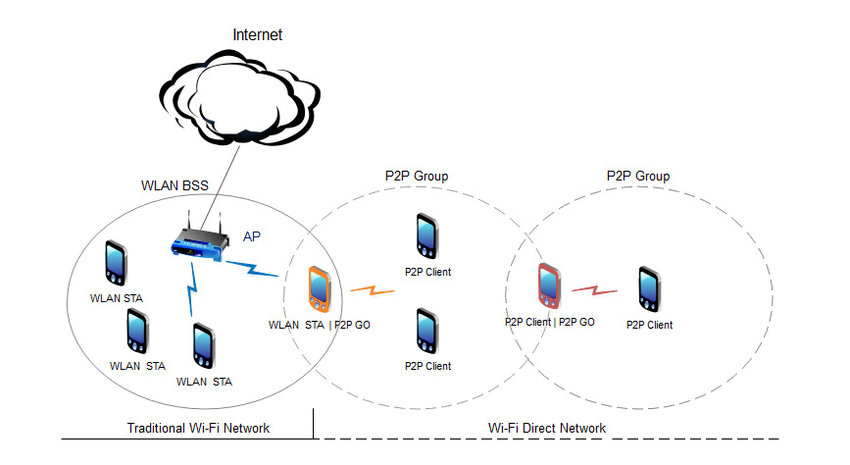
\includegraphics[width=1\columnwidth]{imgs/wifip2pnet.jpg} % Example image
\end{figure}


\label{sec:sezioni}
Wi-Fi Alliance ha introdotto nel 2010 la tecnologia Wi-Fi Direct per consentire
ai dispositivi
Wi-Fi di connettersi direttamente tra loro senza connettersi a un Access Point
(AP). Wi-Fi Direct,
inizialmente chiamato WiFi Peer-to-Peer (Wi-Fi P2P), è basato sulla modalità
dell'infrastruttura
IEEE 802.11 e offre una comunicazione dispositivo-dispositivo diretta, sicura e
rapida. Il recente
Wi-Fi P2P Technical Specification \cite{alliance2016wi} è stato rilasciato nel
2016 (versione 1.7).
I dispositivi abilitati Wi-Fi Direct si scoprono e formano un gruppo P2P. In
ciascun gruppo P2P, 
un nodo eletto, chiamato Group Owner (GO) P2P, funge da AP.


Wi-Fi Direct consente a dispositivi Wi-Fi come smartphone, laptop, smart TV, 
stampanti, fotocamere e altri dispositivi di connettersi in modo rapido e
comodo senza 
l'aggiunta di un Access Point (AP). Wi-Fi Direct è basato sulla
l'infrastruttura 
della WLAN. Le connessioni Wi-Fi Direct sono protette 
con Wireless Protected Access - 2 (WPA2) \cite{mathews2007evolution}.
Wi-Fi Direct supporta le stesse elevate velocità di trasmissione dati del Wi-Fi
(fino a 250 Mbps).
La portata della connessione Wi-Fi Direct è di 200 metri (questa è la portata
teorica e la portata
pratica potrebbe essere minore). Le specifiche richiedono inoltre una
connessione 
1: 1 obbligatoria per i dispositivi certificati Wi-Fi Direct, in cui mantenere
la funzione 
opzionale 1: N. Nelle sezioni successive, 
forniamo una panoramica dettagliata delle funzionalità Wi-Fi Direct.



\section{Architettura di rete}



L'entità funzionale dell'architettura Wi-Fi Direct è denominata 
"Gruppo P2P" che è funzionalmente equivalente a un Basic Service Set
(BSS) nella rete Wi-Fi legacy. Un gruppo P2P è costituito da un proprietario
di un gruppo P2P (P2P GO) e zero o più client P2P. Il P2P GO
è anche chiamato Soft-AP. Le funzioni AP sono implementate nei dispositivi P2P
Wi-Fi. 
Un dispositivo P2P può assumere dinamicamente il ruolo di un AP o di un client.
I ruoli
dei dispositivi P2P (ad esempio P2P GO e P2P Client) vengono solitamente
negoziati prima
di creare un gruppo P2P e rimangono fissi mentre il gruppo P2P è attivo. La
Figura 2.1 illustra
i diversi ruoli dei dispositivi P2P.



\section{Device Discovery}




Device Discovery è una funzione obbligatoria che deve essere supportata
da tutti i dispositivi P2P. Prima di formare un gruppo P2P, un dispositivo 
P2P esegue la procedura Rilevamento dispositivo per rilevare la presenza di
altri dispositivi P2P nel suo intervallo wireless. La procedura consiste in
due fasi distinte: Scansione e Trova. Nella fase di scansione, il dispositivo
P2P esegue la tradizionale scansione Wi-Fi (scansione passiva) attraverso 
tutti i canali supportati al fine di raccogliere informazioni sui dispositivi 
circostanti, i gruppi P2P e le reti Wi-Fi legacy. Una volta completata la
fase di scansione, il dispositivo entra nella fase di ricerca. Nella 
fase di ricerca, il dispositivo P2P si alterna tra due stati: Cerca
e Ascolta. Nello stato Cerca, il dispositivo P2P invia uno o più 
frame Probe Request (PREQ)

sul canale social, ovvero i canali 1, 6 e 11 nella banda dei 2,4 GHz.
Nello stato di ascolto, il dispositivo P2P si sofferma su uno dei canali
social (1, 6 e 11) chiamato canale Listen e attende i frame Probe Request
(PREQ) da altri dispositivi P2P. Quindi, il successo della fase di ricerca 
è quello in cui due dispositivi arrivano a un canale comune per comunicare.
È evidente che il processo di Rilevamento dispositivo P2P può indurre 
qualche ritardo a un dispositivo P2P per scoprire tutti i 
dispositivi P2P nella sua posizione iniziale. Questo ritardo, definito 
"Ritardo rilevamento dispositivo", può essere relativamente elevato se 
diversi dispositivi P2P eseguono contemporaneamente Rilevamento dispositivo
nello stesso intervallo wireless. La figura 2.2 illustra la procedura di 
rilevamento dei dispositivi P2P in Wi-Fi Direct.

\begin{figure}
\caption{Fase di discovey}
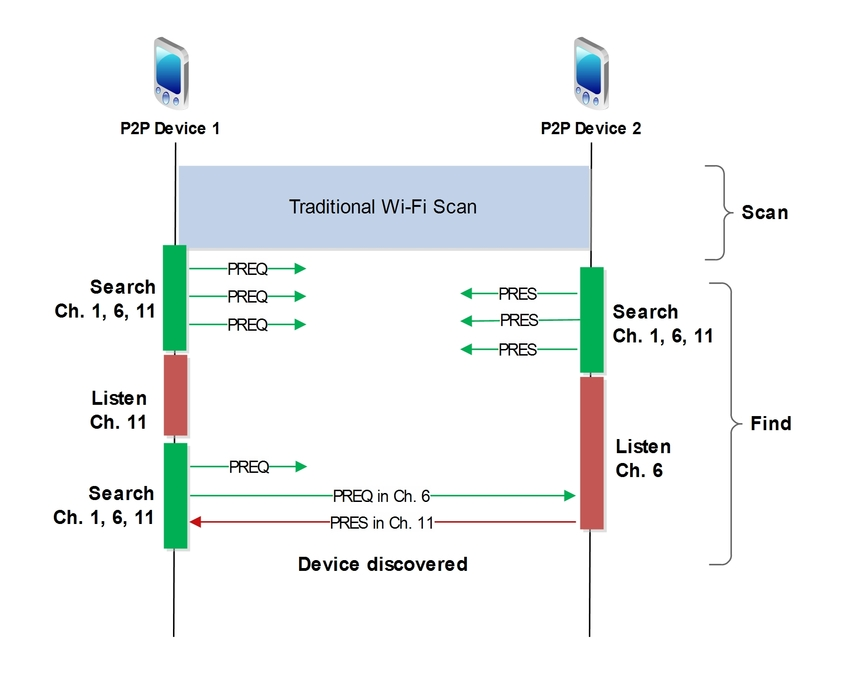
\includegraphics[width=1\columnwidth]{imgs/DeviceDiscovery.jpg} % Example image
\end{figure}


\section{Service Discovery}
Service Discovery è una
procedura opzionale in Wi-Fi Direct. La procedura inizia dopo il 
rilevamento dei dispositivi e prima della procedura di formazione dei 
gruppi. Consente a un dispositivo P2P di connettersi ad altri dispositivi
P2P solo se quest'ultimo fornisce il servizio previsto. Utilizzando la 
procedura di individuazione del servizio, un dispositivo P2P pubblicizza
i servizi disponibili utilizzando il protocollo GAS 
(Generic Advertisement Service) \cite{wikipedia_2015}. 
Wi-Fi Alliance ha definito una serie di servizi standard supportati
da Wi-Fi Direct come Play, Send e Print \cite{wi-fialliance}





\section{Formazione Gruppi}

In seguito al successo di Device Discovery (procedura obbligatoria) e
Service Discovery (procedura facoltativa), i dispositivi P2P  possono
stabilire il gruppo P2P. Durante la Formazione di gruppo, il dispoitivo
sarà GO sarà determinato . Come descritto in Figura 2.3 ci sono 
tre schemi di formazione dei gruppi P2P possibili in

Wi-Fi Direct: (1) Formazione di gruppo standard (2) Formazione di 
gruppi autonomi e (3) Formazione di gruppi permanenti. Nella formazione 
di gruppi standard, presentata nella figura 2.3,  due dispositivi P2P
negozieranno
tra loro il chi sarà GO . La negoziazione del GO è un handshake a 
tre vie. Durante l'handshake, i due dispositivi inviano tra loro un valore
numerico scelto a caso chiamato "Intent value". L'Intent value
va da 0 a 15 e misura il desiderio del dispositivo P2P di essere il P2P 
GO. Il dispositivo P2P che invia il valore di Intento più elevato 
diventa GO.Nel caso in cui entrambi i dispositivi inviano
lo stesso Intent value, viene utilizzato 
un bit di breaker per la decisione e il dispositivo con il bit breaker   
impostato a uno diventa il GO.

\begin{figure}
\caption{tipi di gruppi Wi-Fi Direct}
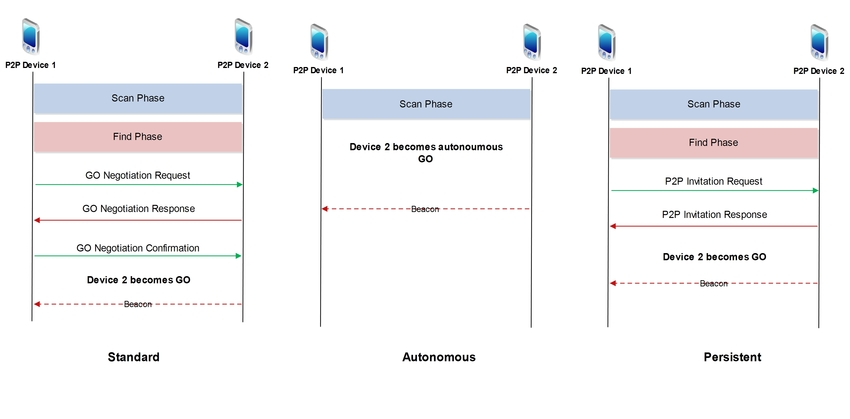
\includegraphics[width=1\columnwidth]{imgs/wifiGroup.jpg} % Example image
\end{figure}


La Figure 2.4 mostra il confronto del valore
dell'Intent tra due dispositivi P2P durante la Formazione di gruppi 
standard. Il dispositivo P2P selezionato come P2P GO avvierà una
sessione di gruppo P2P. L'altro dispositivo P2P può quindi
connettersi al P2P GO per ottenere credenziali e scambiare
dati. Allo stesso modo, altri dispositivi P2P e dispositivi
Wi-Fi legacy possono unirsi al gruppo P2P come client. Nella
formazione di gruppi autonomi, illustrata nella figura 2.3,
il ruolo di GO non è negoziato. Un dispositivo P2P 
si annuncia come GO e inizia a inviare i beacon. Questo
processo è molto simile al Wi-Fi legacy in cui un AP 
invia direttamente Beacons nella rete per diventare
rilevabile. La formazione di gruppi autonomi è più
semplice e più veloce della formazione di gruppi
standard. nella formazione di gruppi persistenti, come illustrato 
nella figura 2.3, un dispositivo P2P invia un invito
a un altro dispositivo P2P, precedentemente collegato
ad esso in un gruppo P2P, per ristabilire il gruppo P2P. 
Questo si ottiene usando i frame Invitation Request e P2P
Invitation Response di P2P. Il ruolo di ciascun dispositivo
P2P deve rimanere uguale a quello del gruppo P2P precedentemente
formato. 
\begin{figure}
\centering
\caption{comparazione Intent Value}
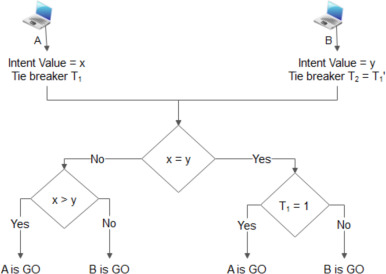
\includegraphics[width=0.9\columnwidth]{imgs/intentValueComparison.jpg} %
%Example image

\end{figure}
Per stabilire un gruppo persistente, i dispositivi P2P
devono dichiarare il gruppo P2P come persistente durante la formazione
standard o autonoma del gruppo.
dei flag bit all'interno dei beacon P2P,dei telegrammi Probe 
Response e nella GO Negotiation vengono utilizzati 
per indicare che il gruppo P2P è persistente o no. 
Se il flag bit non è impostato durante la procedura di formazione dei
gruppi, i dispositivi P2P non possono riattivare un gruppo persistente
in futuro e devono avviare un gruppo standard o autonomo. La specifica
Wi-Fi Direct \cite{alliance2016wi} definisce le procedure di formazione di
gruppi standard
e permanenti solo tra due dispositivi P2P. Gli altri dispositivi P2P i ricerca
possono essere aggiunti, a gruppi P2P formati in precedenza.



\section{Sicurezza}

Wi-Fi Direct richiede a tutti i dispositivi P2P di 
implementare Wi-Fi Protected Setup (WPS) \cite{WPS} al fine di
proteggere il processo di creazione della connessione e della
la comunicazione nel Gruppo P2P. Nello schema WPS, il 
P2P GO implementa il Registrar interno in cui il client 
P2P implementa Enrollee. Lo schema WPS funziona in due fasi.
Nella fase 1, il Registrar interno genera e invia le credenziali 
di rete per iscriversi. Nella fase 2, l'inscritto (Client P2P) 
si ricollega al Registrar interno (P2P GO) utilizzando le 
nuove credenziali



\section{Risparmio energetico}

Il Wi-Fi legacy utilizza il risparmio energetico utilizzando le modalità
Sleep e Active per gli STA Wi-Fi (client). La maggior parte degli AP 
tradizionali sono permanentemente collegati a una normale fonte di 
alimentazione e, quindi, non hanno bisogno di alcuna funzione di risparmio 
energetico. Tuttavia, in Wi-Fi Direct, il P2P GO, che funge da Soft-AP,
può essere un dispositivo alimentato a batteria e ha una durata limitata.
Quindi,
Wi-Fi Direct introduce due nuovi schemi per il risparmio energetico nei 
dispositivi P2P. Questi schemi sono: (1) Opportunistic Power Save
(OppPS) e (2) Notice of Absence (NoA). Nello schema OppPS, il GO è 
autorizzato a risparmiare energia quando i suoi clienti sono in 
modalità Sleep. Il GO annuncia il suo periodo di presenza chiamato 
"CTWindow". Alla fine della CTWindow, se tutti i nodi sono in modalità 
Sleep, il GO può anche andare in modalità Sleep fino al prossimo Beacon.
Tuttavia, alla fine della CTWindow, se uno dei nodi Client P2P è in 
modalità attiva, il GO deve rimanere attivo fino al prossimo beacon.
Nello schema NoA, il GO annuncia tramite i frame Beacons e Probe
Response, un "periodo di assenza". Durante il periodo di assenza,
i suoi client non possono accedere al canale, quindi il GO spegne 
la sua radio per risparmiare energia utilizzata in trasmissione o 
ricezione. Il periodo di assenza viene annunciato in Beacons 
utilizzando NoAschedule, costituito da quattro parametri: 1) 
Durata - la durata del periodo di assenza, 2) Intervallo - il 
tempo tra due periodi di assenza consecutivi, 3) Ora inizio - 
l'ora di inizio del primo periodo di assenza dopo l'attuale Beacon 
e 4)  Count: il numero di periodi di assenza nel 
NoA scheduling corrente. La specifica Wi-Fi Direct non 
definisce i valori di questi parametri.




\chapter{App messaggistica in Wi-fi Direct}

\begin{minipage}{12cm}\textit{
    In questo studio 
    di tesi è stata sviluppata un'app per
   dispositivi android che prevede lo scambio di
    messaggi criptati tra due dispositivi,
   nei paragrafi seguenti andremo a illustrarne il 
   funzionamento e analizzeremo
   i principali limiti del Wi-Fi Direct in android.}
\end{minipage}




\section{Wi-Fi Direct in android}

Google ha annunciato il supporto Wi-Fi Direct su Android 4.0 (livello API 14)a ottobre 2011
\cite{wikiDi} e si trova su tutte le versione di android successive.
Le specifiche del Wi-fi Direct, come abbiamo visto nel capitolo 3,
non vietano ad un dispositivo di partecipare a più gruppi contemporaneamente.
Tuttavia allo stato attuale in Android  un dispositivo non
può far parte di due o più gruppi
nello stesso istante di tempo,
di conseguenza se ci si vuole connettere a un'altro gruppo
bisogna disconnettersi da quello a cui si è connessi, riavviare la fase di discovery
e connettersi a gruppo desiderato.
Il Wi-Fi P2P su Android a livello implementativo, è composto da un insieme di
funzioni disponibili al programmatore, chiamate API e che sono divise in tre parti
principali:
\begin{figure}
   \centering
   \caption{metodi principali della classe WifiP2pManager}
   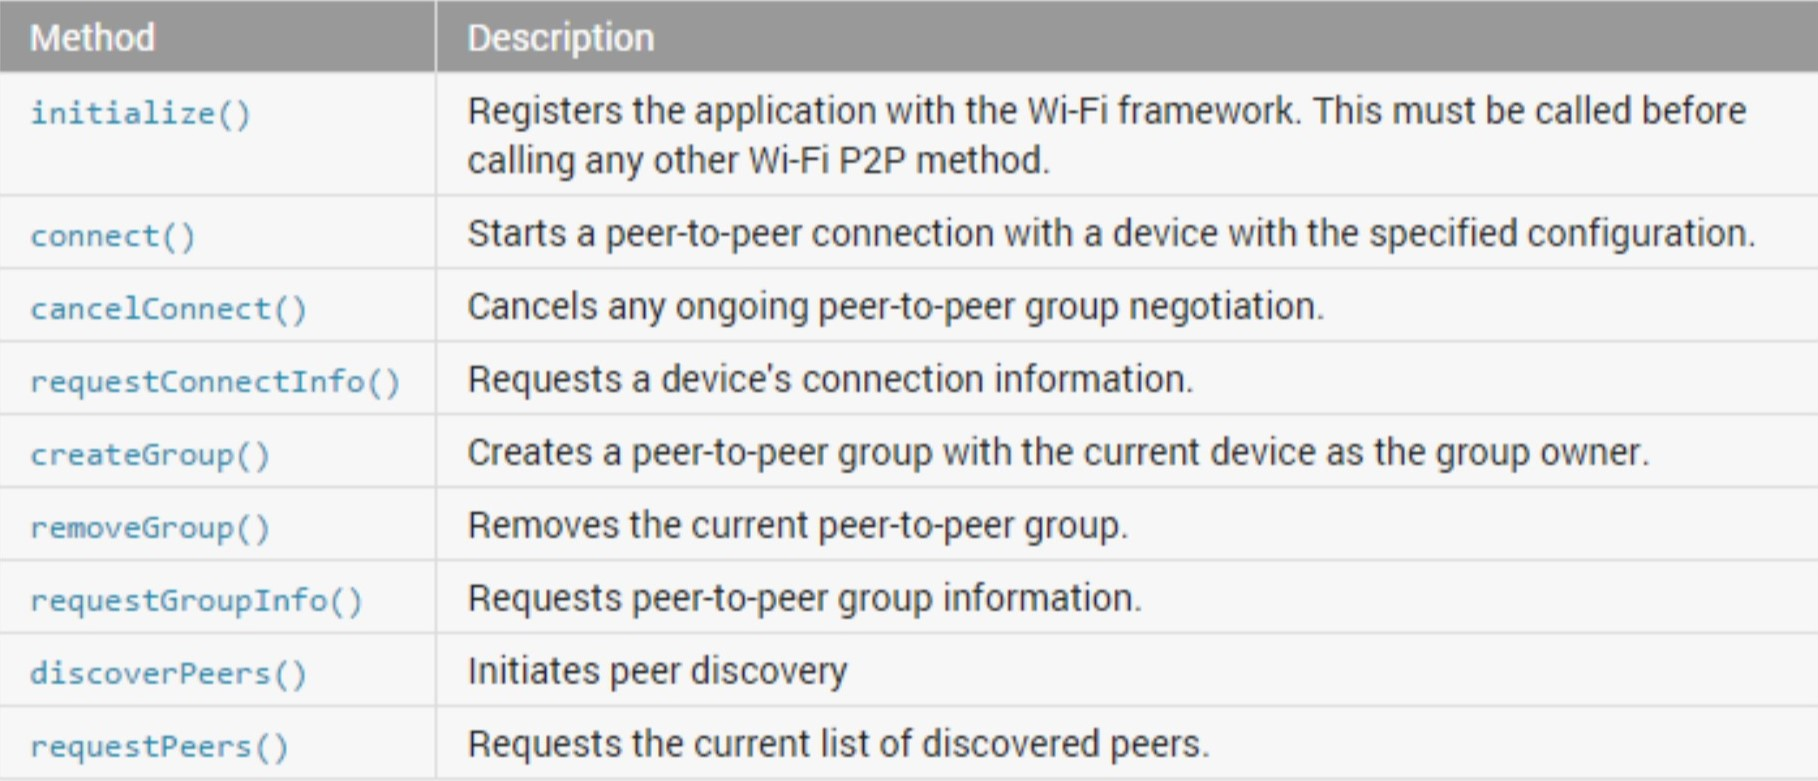
\includegraphics[width=1\columnwidth]{imgs/wifip2pmanagerMet.jpg}
\end{figure}
\begin{itemize}
   \item tutti i metodi definiti nella classe WifiP2pManager che
   consentono la scansione,
   richiesta e connessione con i peer;
   \item i listener, “oggetti” che permettono di notificare
   stati di “successo” o
   “fallimento” quando si eseguono metodi della classe WifiP2pManager;
   \item Intent che notificano ogni
   specifico evento rilevato dal device, ad
   esempio se la connessione cade, se un peer è stato appena scoperto ecc.
\end{itemize}
Qui di seguito in figura, sono esposti i metodi della classe WifiP2pManager.
Ogni metodo della classe WifiP2pManager è collegato a un listener, il quale a
seconda dell’esito della chiamata del metodo, si occupa di avvisare con un
messaggio di successo o fallimento.
Inoltre le API del Wi-Fi P2P definiscono degli intent che, registrati su un
BroadcastReceiver, permettono all’applicazione di rilevare gli eventi che
accadono in un preciso istante.
\begin{figure}
   \centering
   \caption{lista dei listener associati ai vari metodi della classe WifiP2pManager}
   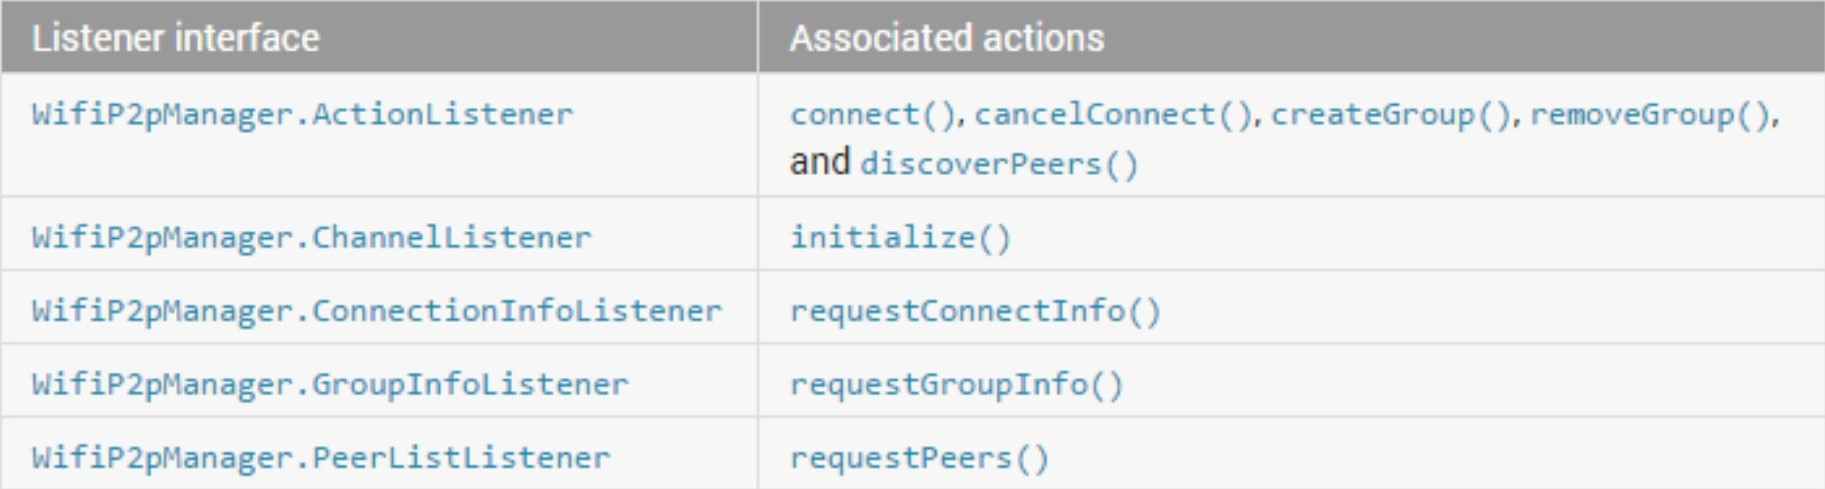
\includegraphics[width=1\columnwidth]{imgs/listenerwifip2pmanager.jpg}
\end{figure}

\section{Funzionamento}

\begin{figure}
   \centering
   \caption{inizio fase di scan}
   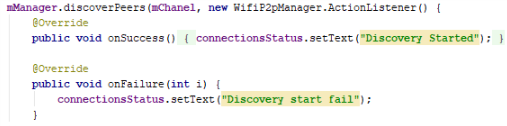
\includegraphics[width=1\columnwidth]{imgs/discoveryStart.png} % Example image
\end{figure}
ho utilizzato le API di Android Software Development Kit (SDK)
in Android Studio \cite{ASD} per lo sviluppo di questa applicazione

\subsection{Descrizione alto livello}

applicazione prevede la comunicazione tra due dispositivi android,
quest'ultimi entrano nella fase di discovery e una volta che si sono trovati
possono instaurare una connessione,
che una volta stabilita aprirà un canale di comunicazione bidirezionale tra i due.
I due dispositivi adesso possono scambiare i messaggi.

\subsection{Fase di scan}

\begin{figure}
   \caption{listener dei peer}
   \centering
   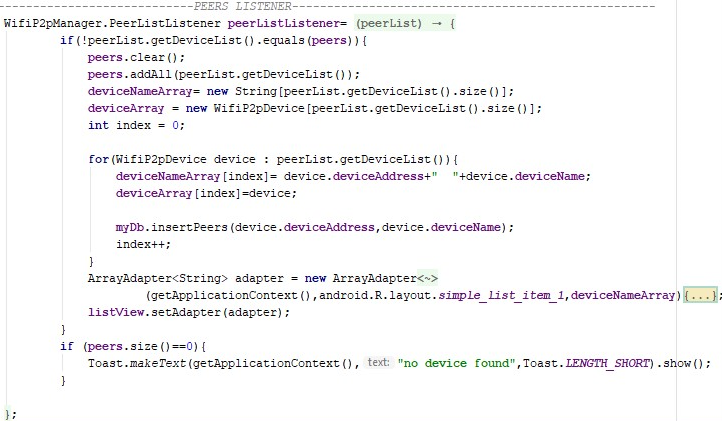
\includegraphics[width=1\columnwidth]{imgs/peerListener.png}% Example image
\end{figure}
per iniziare la fase di scan si utilizza mManager, un
oggetto che abbiamo istanziato nella MainActivity
di tipo WifiP2pManager,questa classe ci fornisce le API per gestire le connessioni
Wi-Fi P2P \cite{androiddevelopers},
come possiamo vedere dalla figura 3.3.
Per ricavare la lista dei peer (dispositivi vicini)
si utilizza un listener,
che ogni volta rileva un nuovo peer lo salva nel suo database
interno al dispositivo e lo
visualizza su schermo insieme agli altri, il codice è mostrato
in figura 3.4

\subsection{Instaurazione della connessione e selezione del Go}

Una volta che l'utente ha su schermo la lista dei dispositivi
vicini può scegliere il dispositivo con il quale comunicare
semplicemente cliccandoci sopra il dispositivo proverà a
connettersi al device selezionato usando il metodo "connect"
della classe "WifiP2pManager" si vede dalla figura 3.5.
\begin{figure}
   \caption{richiesta connessione}
   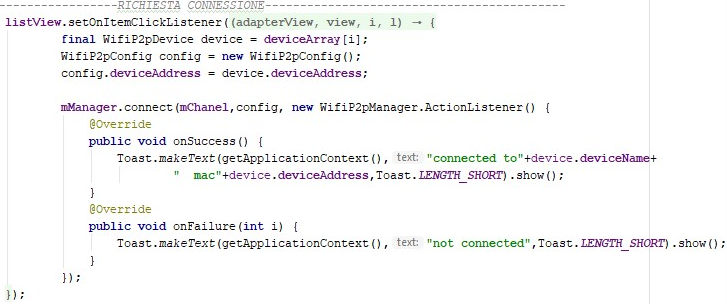
\includegraphics[width=1\columnwidth]{imgs/Connect.png}
\end{figure}
Dopo di che entra in gioco il listener della connessione.
In quest'ultimo verrà scelta la classe da avviare
(client o server)in base al dispositivo che è
diventato GO come si vede nel codice in figura 3.6.
\begin{figure}
   \caption{}
   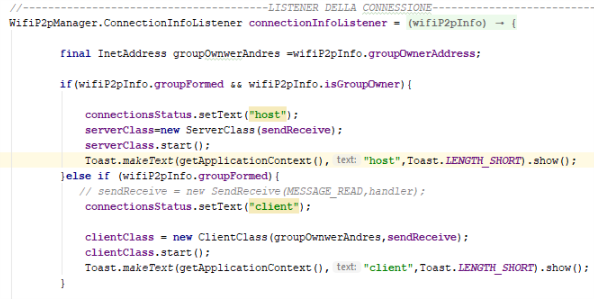
\includegraphics[width=1\columnwidth]{imgs/listenerConeessione.png}
\end{figure}

\subsection{Scambio di messaggi}

\subsubsection{Server Class}

Nel caso al dispositivo assume il ruolo del GO
viene istanziato un oggetto della  classe ServerClass,
che accetta una connessione sulla porta 8888
attraverso una serverSocket che sarà utilizzata per comunicare
attraverso la classe SendReceive come vedremo più avanti
\begin{figure}
   \caption{server class}
   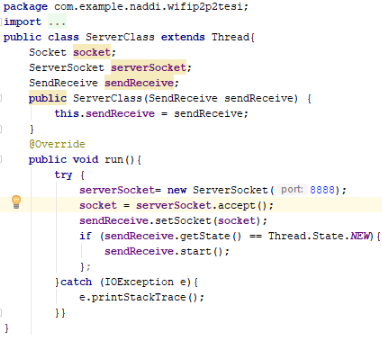
\includegraphics[width=0.8\columnwidth]{imgs/serverClass.png}
   \centering
\end{figure}

\subsubsection{Client Class}

Invece nel caso il dispositivo non assume il ruolo del GO
viene istanziato un oggetto della classe ClientClass,
che prova a connettersi all'indirizzo del GO sulla porta 8888 attraverso
una socket che sarà utilizzata per comunicare
attraverso la classe SendReceive come vedremo più avanti.
\begin{figure}
   \caption{client class}
   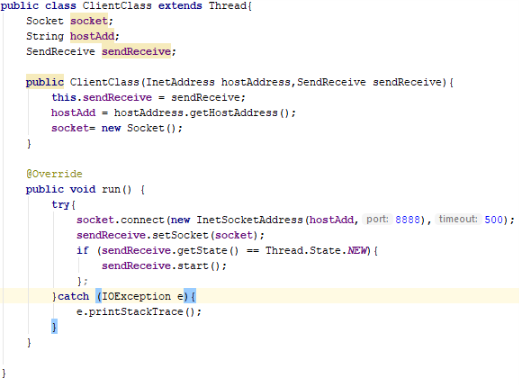
\includegraphics[width=1\columnwidth]{imgs/clientClass.png}
   \centering
\end{figure}


\subsubsection{Scambio di messaggi attraverso SendReceive}

SendReceive si occupa di inviare i messaggi all'altro dispositivo
e di riceverli;
per inviarli utilizza il metodo write che scrive
sull'output stream della socket
per riceverli controlla continuamente l'input stream
della socket


\subsection{Crittografia usata}

Sebbene Wi-Fi Direct utilizza  che usa una crittografia di tipo
AES \cite{Wi-FiProtected}
nell'app si è voluto aggiungere un ulteriore layer di crittografia
implementato a livello software.
Per criptare i messaggi è stata usata la libreria
Spongy Castle \cite{Spongy} questa libreria è stata derivata
da Bouncy Castle in quanto 
la piattaforma Android sfortunatamente viene
distribuita con una versione ridotta di Bouncy Castle,
Spongy Castle è uguale a Bouncy Castle
ma con un paio di piccole modifiche per farlo funzionare su Android.
per generare la coppia di chiavi ho usato la curva ellittica con parametri
(Standards for Efficient Cryptography)
"secp224k1" \cite{sec}.
Per gestire la crittografia è stata creata una classe Cript che contiene
gli oggetti e i metodi necessari per essa: la coppia di chiavi pubblica e privata
del dispositivo e la chiave pubblica dell'altro dispositivo; per quanto riguarda i metodi
invece ce ne sono 4:
\begin{itemize}
   \item Cript() è il costruttore della classe Cript e
   inizializza la coppia di chiavi pubblica e privata.
   \begin{figure}
       \caption{costruttore della classe Cript}
       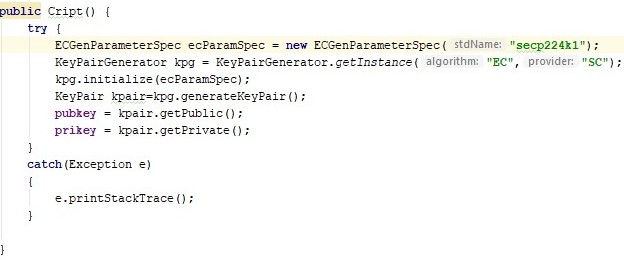
\includegraphics[width=1\columnwidth]{imgs/Criptconstructor.jpg}
   \end{figure}
   \item setHisKey() prende in input la chiave pubblica dell'altro dispositivo
   encodata in base64 ne fa il decode la memorizza all'interno dell'oggetto
   nel campo "hispub".
   \begin{figure}
       \caption{setter del campo hispub}
       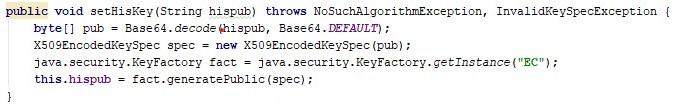
\includegraphics[width=1  \columnwidth]{imgs/sethiskey.jpg}
   \end{figure}
  \item encript() prende in input il messaggio da criptare e lo cripta con la
   chiave pubblica dell'altro dispositivo e ritorna il messaggio criptato
   encodato in base64.
   \begin{figure}
       \caption{metodo per criptare il messaggio}
       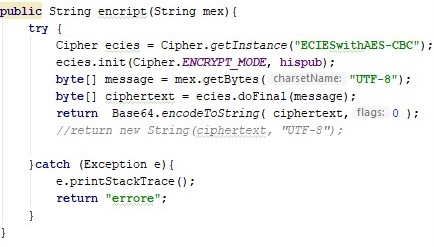
\includegraphics[width=0.8  \columnwidth]{imgs/encript.jpg}
   \end{figure}
   \item decript() prende in input il messaggio da decriptare encodato in base64
   e lo decripta con
   la sua chiave privata e ritorna il messaggio decriptato.
   \begin{figure}
       \caption{metodo per decriptare il messaggio}
       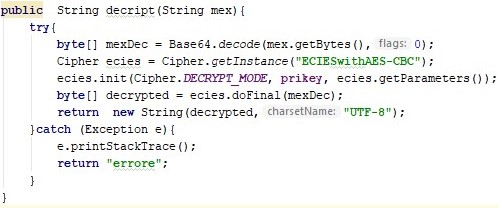
\includegraphics[width=1  \columnwidth]{imgs/decript.jpg}
   \end{figure}
\end{itemize}

\subsubsection{scambio chiavi pubbliche dei dispositivi}

Una volta che I dispositivi si sono connessi e hanno istanziato
rispettivamente la classe server e client sono pronti a scambiarsi i messaggi
e il primo messaggio che si scambiano in modo automatico è la loro chiave pubblica
questo senza che l'utente si accorga di nulla.
la coppia di chiavi pubblica e privata vengono generate a ogni nuova connessione.

\section{Analisi del Wi-Fi Direct}

Dall'esperienza acquisita sviluppando questo prototipo di app è emerso
che il Wi-Fi Direct risulta ottimo per connettere i dispositivi singolarmente
fornendo velocità di trasmissione standard del wifi questa cosa è stata confermata
anche dai test effettuati sul campo che mostreremo più avanti,
mentre non è adatto a formare una rete di dispositivi connessi in quanto
come in android non è permessa la connessione  
del dispositivo a due Gruppi differenti (cosa che nello standard non è limitata) 
nello stesso momento,
nel senso un dispositivo che è connesso a un Gruppo "A" 
e desidera connettersi a un gruppo "B"  si deve disconnettere da "A" e connettersi a "B";
di conseguenza non può neanche fare da ponte di comunicazione tra i due gruppi.
Dai test sul campo ivece si è osservato che il tempo di discovery e quello di formazione del gruppo
hanno mostrato risultati discordanti in quanto con l'aumento della distanza quest'ultimi
impiegavano meno tempo, si noti però che durante lo sviluppo dell'app di messaggistica
in alcuni casi la fase di discovery è arrivata a richiedere anche più 10 secondi risultando 
però soddisfacenti nella maggioranza dei casi.
I test che ho fatto inoltre hanno mostrato il limite della portata
del Wi-Fi Direct si è osservato che fino a 64 metri
(all'aperto e senza ostacoli) i dispositivi
si connettevano e riuscivano a scambiare messaggi  mentre a 128 metri
mentri sebbene i disponibili si vedessero (con difficoltà) non riuscivano
a stabilire una connessione non riuscendo quindi neanche a scambiarsi messaggi,
per questo motivo i test a questa distanza non sono stati riportati nella tabella.
Di seguito riporteremo i vari test sulle varie distanze con i tempi (in secondi)di:
discover,group formation,e trasferimento di un payload da 10MByte.
Un altro limite del Wi-Fi Direct è il consumo di una batteria che risulta
essere elevato.

\subsubsection{I test effettuati}

I test sono stati effettuati attraverso un'app sviluppata da me
su due dispositivi rispettivamente,
uno xiaomi redmi 5 pro e uno xiaomi redmi note 6, pro dove tengo
traccia rispettivamente del tempo che i due dispositivi impiegano a
trovarsi, il tempo di formazione del gruppo e il tempo che impiegano
per inviare una payload di 10 MByte.
I test sono stati eseguiti per le seguenti distanze in metri 0,4,8,16,64,128
per ogni distanza il test è stato eseguito 5 volte
i valori che riporteremo sono la risultante della media dei 5.
il test viene eseguito nel seguente: modo chiameremo d1 il dispositivo 1
e d2 il dispositivo 2,
d2 entra per primo in modalità discovery dopo di che anche d1 entra in modalità
discovery adesso il tempo che d1 impiega per trovare d2 sarà il tempo
di discovery che viene registrato. Per tempo di formazione del
gruppo si intende il tempo che uno dei due dispositivi impiega a
diventare Group owner, una volta che i dispositivi sono connessi
si procede con l'invio del payload e registrazione del tempo impiegato.

%https://www.tablesgenerator.com/latex_tables
\begin{table}
   \centering
   \begin{tabular}{|c|c|c|c|}
   \hline
   \begin{tabular}[c]{@{}c@{}}Distanze\\ in\\ metri\end{tabular} & \begin{tabular}[c]{@{}c@{}}Tempo \\ (in secondi)\\ Discovery\end{tabular} & \begin{tabular}[c]{@{}c@{}}Tempo\\ (in secondi)\\ formazione\\ gruppo\end{tabular} & \begin{tabular}[c]{@{}c@{}}Tempo\\ (in secondi)\\ invio\\ payload \\ di 10 Mbyte\end{tabular} \\ \hline
   0                                                             & 2.42                                                                      & 1.84                                                                               & 2.5                                                                                           \\ \hline
   4                                                             & 1.45                                                                      & 1.27                                                                               & 5.25                                                                                          \\ \hline
   8                                                             & 1.04                                                                      & 0.94                                                                               & 5.8                                                                                           \\ \hline
   16                                                            & 0.1                                                                       & 1.44                                                                               & 12.4                                                                                          \\ \hline
   32                                                            & 4,6                                                                       & 1.6                                                                                & 14,6                                                                                          \\ \hline
   64                                                            & 1,12                                                                      & 1.42                                                                               & 17,6                                                                                          \\ \hline
   \end{tabular}
   \end{table}

   \chapter*{Conclusioni}
   In questa tesi inizialmente si è visto cosa è una Near-Me area network e
   si è fatta una panoramica sulle reti peer to peer come si correlassero 
   con il Wi-fi Direct; successivamente siamo andati ad approfondire le specifiche
   dello standard del Wi-Fi Direct andando ad analizzarne il
    funzionamento vero e proprio.
   Dopo questa parte si è passati allo studio del Wi-Fi Direct
   in android e la spiegazione dell'implementazione
   proposta di un'app , sviluppata per questo studio di tesi,
   che usa il Wi-Fi Direct per lo scambio di messaggi
   tra due dispositivi.
   Successivamente siamo andati a testare le performance del Wi-Fi Direct
   attraverso un'altra app sviluppata appositamente per lo scopo.
   Da questo studio di tesi è emerso che allo stato attuale
   non è possibile costruire una rete peer to peer
   attraverso il Wi-Fi Direct ma più tosto è più orientato
   per connessioni peer to peer.










%\chapter{Conclusioni e sviluppi futuri}

Inserire qui le conclusioni trovate con la tesi, ed eventualmente eventuali idee per sviluppi futuri.
\chapter*{Appendice A}

Qui di seguito sono elencati i link ai codici sorgenti degli applicativi utilizzati
nella tesi e della tesi stessa

\subsubsection{codice latex di questa tesi:}

\url{https://github.com/naddi96/Il-Wi-Fi-Direct-per-le-reti-peer-to-peer-un-prototipo-di-applicazione-near-me-area-network-e-analis}

\subsubsection{app messagistica:}

\url{https://github.com/naddi96/-messaging-app-using-Wi-Fi-Direct}

\subsubsection{app usata per i test:}

\url{https://github.com/naddi96/app-for-testing-Wi-Fi-Direct-}






% ELENCO DELLE FIGURE (OPZIONALE)
\addcontentsline{toc}{chapter}{Elenco delle figure}
\listoffigures


% BIBLIOGRAFIA

\addcontentsline{toc}{chapter}{Bibliografia}

\bibliography{citation}{}
\bibliographystyle{ieeetr}
%\bibliographystyle{plain}




\end{document}